\chapter{MFCC dan Neural Network}

\section{Teori}
\begin{enumerate}
\item Kenapa file suara harus di lakukan MFCC. dilengkapi dengan ilustrasi atau gambar. 
\par Nilai-nilai MFCC meniru pendengaran manusia dan mereka biasanya digunakan dalam aplikasi pengenalan suara serta genre musik
deteksi. Nilai-nilai MFCC ini akan dimasukkan langsung ke jaringan saraf.Agar dapat diubah menjadi bentuk vektor, dan dapat digunakan pada machine learning. Disebabkan machine learning hanya mengerti bilangan vektor saja.
Ilustrasinya, Ketika ingin menggunakan file suara dalam machine learning, misalnya untuk melihat jam. Machine learning tidak memahami rekaman suara melainkan vektor. Maka rekaman tersebut akan diubah kedalam bentuk vektor kemudian vektor akan menyesuaikan dengan kata kata yang sudah disediakan. Jika cocok maka akan mengembalikan waktu yang diinginkan

\item Konsep dasar neural network dilengkapi dengan ilustrasi atau gambar
\par Neural Network ini terinspirasi dari jaringan saraf otak manusia. Dimana setiap neuron terhubung ke setiap neuron di lapisan berikutnya. Lapisan pertama menerima input dan lapisan terakhir memberikan keluaran. Struktur jaringan, yang berarti jumlah neuron dan koneksinya, diputuskan sebelumnya dan tidak dapat berubah, setidaknya tidak selama training. Juga, setiap input harus memiliki jumlah nilai yang sama. Ini berarti bahwa gambar, misalnya, mungkin perlu diubah ukurannya agar sesuai dengan jumlah neuron input.

Ilustrasinya. misalkan kita ingin encode sebuah kalimat yaitu "what time is it" kemudian Anda menginisialisasi lapisan jaringan Anda dan hidden statel. Bentuk dan dimensi hidden state akan tergantung pada bentuk dan dimensi jaringan saraf berulang Anda. Kemudian Anda mengulangi input Anda, meneruskan kata danhidden state ke NN. NN mengembalikan output dan kondisi tersembunyi yang dimodifikasi. Anda terus mengulang sampai Anda kehabisan kata-kata. Terakhir Anda melewatkan output ke layer feedforward, dan itu mengembalikan prediksi. Bahwa kita ingin mengetahui pukul berapa sekarang.

\item Konsep pembobotan dalam neural network.dilengkapi dengan ilustrasi atau gambar
\par Bobot mewakili kekuatan koneksi antar unit. Jika bobot dari node 1 ke node 2 memiliki besaran lebih besar, itu berarti bahwa neuron 1 memiliki pengaruh lebih besar terhadap neuron. 2. Bobot penting untuk nilai input. Bobot mendekati nol berarti mengubah input ini tidak akan mengubah output. Bobot negatif berarti meningkatkan input ini akan mengurangi output. Bobot menentukan seberapa besar pengaruh input terhadap output. Seperti contoh berikut :
\begin{figure}[ht]
\centering
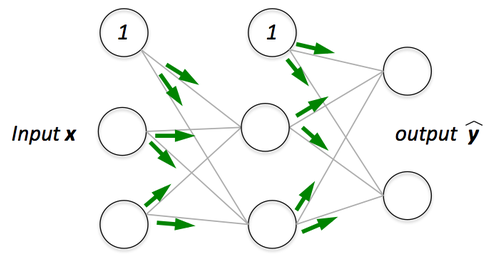
\includegraphics[scale=0.5]{figures/chapter6tasya2.png}
\caption{Contoh Pembobotan Neural Network Tasya}
\label{Teori}
\end{figure}

\item Konsep fungsi aktifasi dalam neural network. dilengkapi dengan ilustrasi atau gambar
\par Fungsi aktivasi digunakan untuk memperkenalkan non-linearitas ke jaringan saraf. Ini menekan nilai dalam rentang yang lebih kecil yaitu. fungsi aktivasi Sigmoid memeras nilai antara rentang 0 hingga 1. Ada banyak fungsi aktivasi yang digunakan dalam industri pembelajaran yang dalam dan ReLU, SeLU dan TanH lebih disukai daripada fungsi aktivasi sigmoid. Ilustrasinya, ketika fungsi aktivasi linier, jaringan saraf dua lapis mampu mendekati hampir semua fungsi. Namun, jika fungsi aktivasi identik dengan fungsi aktivasi F (X) = X), properti ini tidak puas, dan jika MLP menggunakan fungsi aktivasi yang sama, seluruh jaringan setara dengan jaringan saraf lapis tunggal.

\item Cara membaca hasil plot dari MFCC,dilengkapi dengan ilustrasi atau gambar
Berikut merupakan hasil plot dari rekaman suara :
\begin{figure}[ht]
\centering
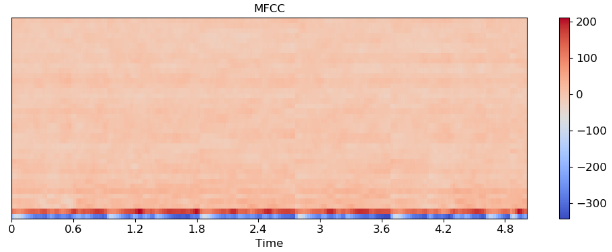
\includegraphics[scale=0.5]{figures/chapter6tasya1.png}
\caption{Cara Membaca Hasil Plot MFCC Tasya}
\label{Teori}
\end{figure}
Dari gambar tersebut dapat diketahui :
\begin{itemize}
\item Terdapat 2 dimensi yaitu x sebagai waktu, dan y sebagai power atau desibel.
\item Dapat dilihat bahwa jika berwarna biru maka power dari suara tersebut rendah, dan jika merah power dari suara tersebut tinggi
\item Dibagian atas terdapat warna merah pudar yang menandakan bahwa tidak ada suara sama sekali dalam jangkauan tersebut.
\end{itemize}

\item Jelaskan apa itu one-hot encoding,dilengkapi dengan ilustrasi kode dan atau gambar.
\par One-hot encoding adalah representasi variabel kategorikal sebagai vektor biner. Mengharuskan nilai kategorikal dipetakan ke nilai integer. Kemudian, setiap nilai integer direpresentasikan sebagai vektor biner yang semuanya bernilai nol kecuali indeks integer, yang ditandai dengan 1.
\begin{figure}[ht]
\centering
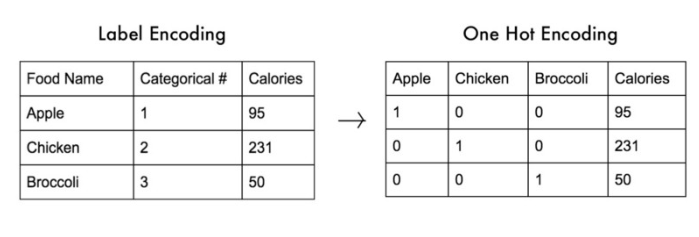
\includegraphics[scale=0.5]{figures/chapter6tasya3.png}
\caption{One Hot Encoding Tasya}
\label{Teori}
\end{figure}

\item fungsi dari np/.unique dan to categorical dalam kode program,dilengkapi dengan ilustrasi atau gambar.
Untuk np unique fungsinya yaitu menemukan elemen unik array. Mengembalikan elemen unik array yang diurutkan. Ada tiga output opsional selain elemen unik:
\begin{itemize}
\item Indeks array input yang memberikan nilai unik
\item Indeks array unik yang merekonstruksi array input
\item Berapa kali setiap nilai unik muncul dalam array input.
\end{itemize}
\begin{figure}[ht]
\centering
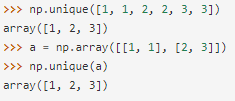
\includegraphics[scale=0.5]{figures/chapter6tasya4.png}
\caption{Numpy Unique Tasya}
\label{Teori}
\end{figure}

Untuk  To Categorical fungsinya untuk mengubah vektor kelas (integer) ke matriks kelas biner.
\begin{figure}[ht]
\centering
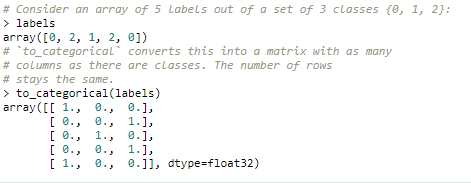
\includegraphics[scale=0.5]{figures/chapter6tasya5.png}
\caption{To Categorical Tasya}
\label{Teori}
\end{figure}

\item Fungsi dari Sequential dalam kode program,dilengkapi dengan ilustrasi atau gambar.
Sequential berfungsi sebagai tumpukan linear lapisan. COntohnya sebagai berikut :
\begin{figure}[ht]
\centering
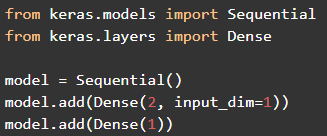
\includegraphics[scale=0.5]{figures/chapter6tasya6.png}
\caption{Sequential Tasya}
\label{Teori}
\end{figure}
\end{enumerate}

\section{Praktek Program}
\subsection{GTZAN Genre Collection dan data dari freesound}
\begin{enumerate}
\item GTZAN Genre Collection berisikan klasifikasi genre musik. Terdapat 1000 audio dengan durasi maksimal 30 detik dan terdapat 10 genre musik didalamnya. Dalam setiap genre berisikan 100 tracks musik.
\item Data dari Freesound berisikan instrument alat musik tertentu dalam bentuk wav
\end{enumerate}
Untuk Meload Data tersebut untuk digunakan pada MFCC caranya dapat dilihat seperti pada listing berikut.
\lstinputlisting[caption=Kode Load Data Untuk MFCC, label={lst:loadingdata}]{src/load_data.tex}
\begin{itemize}
\item PEnjelasannya sebagain berikut :
\item Codingan Diatas akan meload libray librosa yang akan digunakan untuk menggunakan mfcc
\item Librosa\.feature akan meload feature dari librosa
\item Librosa\.display akan mengambil fungsi display pada librosa
\item glob merupakan modul pada python yang digunakan untuk meload segala jenis format file termasuk musik
\item mengimport numpy sebagai np yang digunakan untuk data array dari musik
\item import matplotlib untuk melakukan plotting dari audio
\item Mengimport modul Sequential dari librari Keras untuk membuat suatu model
\item Dense dan Activation sebagai Operasi linier di mana setiap input terhubung ke setiap output dengan bobot atau weight.
\item Dari library keras akan meload modul to\_categorical
\item Kemudian untuk me load datanya, disini variabel audio\_path berisikan direktori file tujuan yang digunakan.
\item Variabel x dan sr berguna untuk meload variabel audio\_path menggunakanlibrari Librosa
\item Kemudia print atau tampilkan x dan s dalam bentuk array.Hasilnya seperti berikut :
\begin{figure}[ht]
\centering
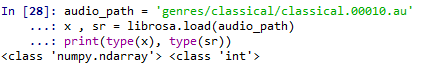
\includegraphics[scale=0.5]{figures/chapter6tasya23.png}
\caption{Meload Data Genre Collection Tasya}
\label{Praktek}
\end{figure}
\end{itemize}

\subsection{Fungsi Display MFCC}
Berikut merupakan Code dari fungsi Display mfcc: 
\begin{figure}[ht]
\centering
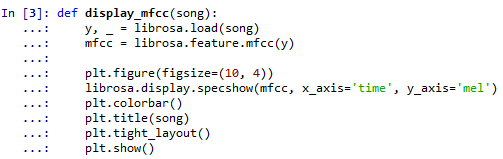
\includegraphics[scale=0.5]{figures/chapter6tasya8.png}
\caption{Display MFCC Tasya}
\label{Praktek}
\end{figure}
Penjelasan dari code diatas yaitu :
\begin{itemize}
\item def display\_mfcc yaitu kita akan mendefinisikan fungsi yang diberinama display\_mfcc dengan inputan song
\item Variabel y akan meload variabel song
\item Variabel MFCC akan menggunakan feauture mfcc pada Librosa untuk melakukan konversi audio menjadi bentuk vektor
\item Kemudian hasil tadi akan diplotting.
\item Berikut merupakan contoh dari plotting audio dari genre Classical. Ketikan kode berikut  yang dimana akan memanggil fungsi dispkay mfcc utuk plotting dari audioyang dituju dapat dilihat dilisting berikut .
\lstinputlisting[caption=Code Fungsi Display MFCC, label={lst:DisplayMFCC}]{src/display_mfcc.tex}
\item Hasilnya sebagai berikut 
\begin{figure}[ht]
\centering
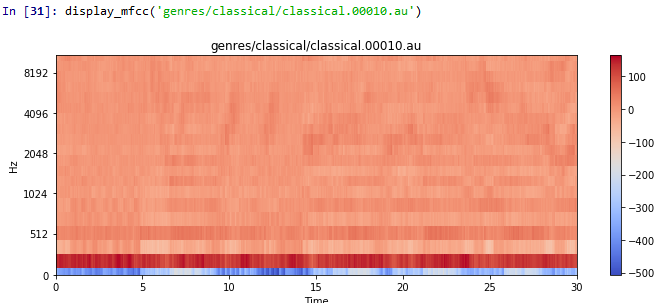
\includegraphics[scale=0.5]{figures/chapter6tasya24.png}
\caption{Hasil Display MFCC Tasya}
\label{Praktek}
\end{figure}
\end{itemize}

\subsection{Fungsi Extract Features Song}
Berikut merupakan code dari fungsi extract features song :
\begin{figure}[ht]
\centering
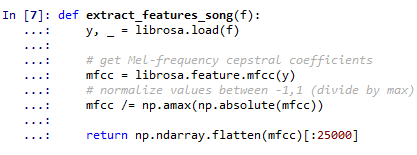
\includegraphics[scale=0.5]{figures/chapter6tasya9.png}
\caption{Extract Features Tasya}
\label{Praktek}
\end{figure}
Penjelasan dari code diatas yaitu :
\begin{itemize}
\item Variabel y akan melaod variabel atau inputan f menggunakan librari Librosa
\item Variabel mfcc akan melakukan mfcc dari variabel y
\item Variabel mfcc kemudian akan dibagi oleh numpy amax dan dikembalikan lagi nilainya ke variabel mfcc.
\item Hasil Tadi kemudian akan ditampilkan dalam bentuk array dengan mengambil 25000 row pertama
\item Mengapa mengambil 25000 row pertama? dikarenakan Audio yang terdapat pada dataset ini tidak menentu durasinya. Dan kita harus mengambil data yang memiliki durasi yang sama untuk mempermudah dalam melakukan training.
\end{itemize}

\subsection{Fungsi Generate Features And Labels}
Berikut merupakan code dari fungsi Generate Features And Labels :
\begin{figure}[ht]
\centering
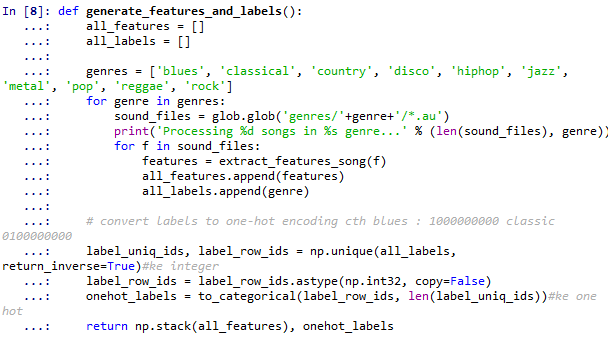
\includegraphics[scale=0.5]{figures/chapter6tasya10.png}
\caption{Fungsi Generate Features And Labels Tasya}
\label{Praktek}
\end{figure}
Penjelasan dari code diatas yaitu :
\begin{itemize}
\item Variabel all features berisikan array kosong
\item Variabel all labels berisikan array kosong
\item Variabel genres disesuaikan dengan nama folder sebelumnya, dan berisikan folder folder dari genre yang ada
\item Melakukan looping, untuk folder tadi
\item Variabel sound\_files akan mengambil file dari folder genres dan mengambil semua file dengan ekstensi au didalamnya.
\item print akan menampilkan Tulisan Prossesing dengan jumlah file didalam folder dan nama folder tersebut
\item Memanggil fungsi extract\_features\_song kedalam inputan f dalam sound\_files dan melakukan vektorisasi dimasukan kedalam variabel features.
\item Semua fitures akan dimasukan kedalam all\_features.
\item Semua genre diamsukan ke all\_labels.
\item Variabel label\_uniq\_ids dan label\_row\_ids mendefinisikan label unique dari all\_labels kedalam bentuk integer.
\item Kemudian variabel onehot\_labels akan mengubahnya ke dalam bentuk one hot encoding dengan menggunakan to\_categorical.Sehingga dimensinya menjadi 1000 x 10 dikarenakan terdapat 1000 lagu dan 10 binari untuk merepresentasikan one-hot encodingnya.
\item Mengembalikan all\_features dan onehot\_labels kedalam satu matriks.
\end{itemize}

\subsection{Penggunaan Fungsi Generate Features And Labels Sangat Lama Ketika Meload Dataset Genre}
\par Dikarenakan TErdapat 10 folder dengan genre berbeda, dan didalamnya terdapat 100 audio. Dari setiap folder itu akan dilakukan features dan perubahan label. Karena banyaknya jumlah file maka proses loadnya pun lama.
Berikut codingannya :
\lstinputlisting[caption=Panggil Genenrate Labels, label={lst:generatelables}]{src/panggil_generatelabel.tex}
Akan didapatkan hasil seperti berikut yang dimana menunujukan proses bahwa sedang dilakukan ektraksi audio ke features dan labels :
\begin{figure}[ht]
\centering
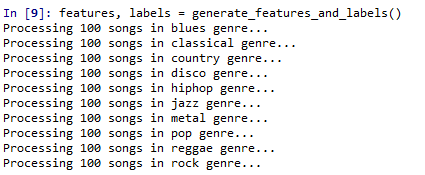
\includegraphics[scale=0.5]{figures/chapter6tasya11.png}
\caption{Hasil Fungsi Generate Features And Labels Tasya}
\label{Praktek}
\end{figure}

\subsection{Pemisahan Data Training Dan Data Set Sebesar 80\%}
\par Pemisahan 80\% digunakan untuk memudahkan dalam melakukan pengacakan atau pengocokan nantinya. Dimana 80\% merupakan data training dan sisanya 20\% merupakan datatestnya. data training perlu lebih banyak agar saat dilakukan pengocokan tidak teracak dalam urutan yang berbeda. Berikut code programnya pada listing ini :
\lstinputlisting[caption=Code Pemisahan Data Training Dan Testing, label={lst:pemisahan}]{src/traintest.tex}
Penjelasan dari code diatas :
\begin{itemize}
\item Training split akan memisahkan training set sebanyak 80\%
\item Melakukan penumpukan features dan labels
\item Melakukan Pengocokan untuk alldata dengan mengalikan isi dari alldata dengan training\_split
\item Memisahkan mana yang termasuk data train dan mana yang termasuk data test
\item Menampilkan isi dari train dan test. Dapat dilihat bahwa untuk training terdapat 800 kolom dan untuk test 200 kolom dengan jumlah baris yang sama yaitu 25010
\begin{figure}[ht]
\centering
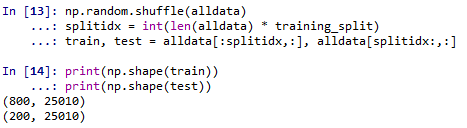
\includegraphics[scale=0.5]{figures/chapter6tasya15.png}
\caption{Pemisahan Data Training dan Data Set Tasya}
\label{Praktek}
\end{figure}
\item Variabel train\_input akan berisikan train dengan mengecualikan 10 baris terakhir
\item Variabel train\_labels berisikan train dengan mengambil sisa dari train\_input atau hanya mengambil 10 baris terakhir saja
\item Untuk variabel test\_input dan test\_label sama penjelasannya seperti diatas.
\item Baris selanjutnya digunakan untuk menampilkan isi atau shape dari hasil training dan testing barusan, seperti berikut :
\begin{figure}[ht]
\centering
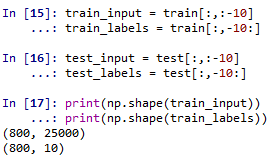
\includegraphics[scale=0.5]{figures/chapter6tasya16.png}
\caption{Pemisahan Data Training dan Data Set Tasya}
\label{Praktek}
\end{figure}
\end{itemize}

\subsection{Fungsi Sequential}
Berikut code lengkapnya :
\lstinputlisting[caption=Code Fungsi Sequential, label={lst:fungsisequential}]{src/sequential.tex}
Hasilnya seperti berikut :
\begin{figure}[ht]
\centering
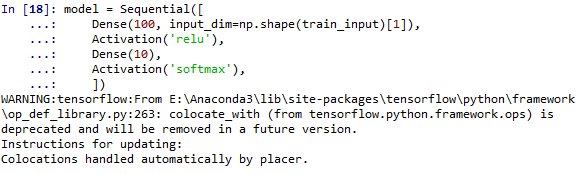
\includegraphics[scale=0.5]{figures/chapter6tasya17.png}
\caption{Pemisahan Data Training dan Data Set Tasya}
\label{Praktek}
\end{figure}
Dari hasil diatas dapat dijelaskan bahwa :
\begin{itemize}
\item Layer pertama dense dari 100 neuron untuk inputan
\item Activationnya menggunakan fungsi relu yaitu jika ada inputan dengan nilai maksimum maka inputan itu yang akan terpilih.
\item Dense 10 mengkategorikan 10 neuron untuk jenis genrenya untuk output nya.
\item Untuk dense diatas aktivasinya menggunakan fungsi Softmax
\end{itemize}

\subsection{Fungsi Compile}
 Berikut code lengkapnya : 
\lstinputlisting[caption=Code Fungsi Compile, label={lst:fungsicompile}]{src/compile.tex}
Hasilnya seperti berikut : 
\begin{figure}[ht]
\centering
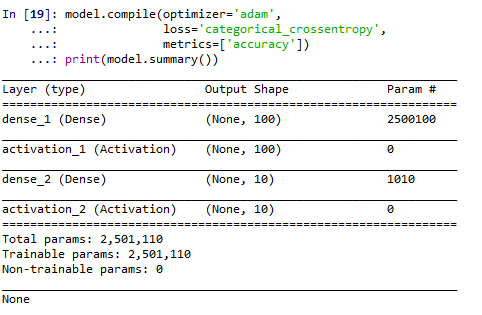
\includegraphics[scale=0.5]{figures/chapter6tasya18.png}
\caption{Fungsi Compile Tasya}
\label{Praktek}
\end{figure}
Dari hasil diatas dapat dijelaskan bahwa :
\begin{itemize}
\item Menggunakan algortima adam sebagai optimizer. Adam yaitu algoritme pengoptimalan yang dapat digunakan sebagai ganti dari prosedur penurunan gradien stokastik klasik untuk memperbarui bobot jaringan yang berulang berdasarkan data training.
\item Loss nya menggunakan categorical\_crossentropy untuk fungsi optimasi skor
\end{itemize}

\subsection{Fungsi Fit}
Berikut code lengkapnya :
\lstinputlisting[caption=Code Fungsi Fit, label={lst:fungsifit}]{src/fit.tex}
Hasilnya seperti berikut :
\begin{figure}[ht]
\centering
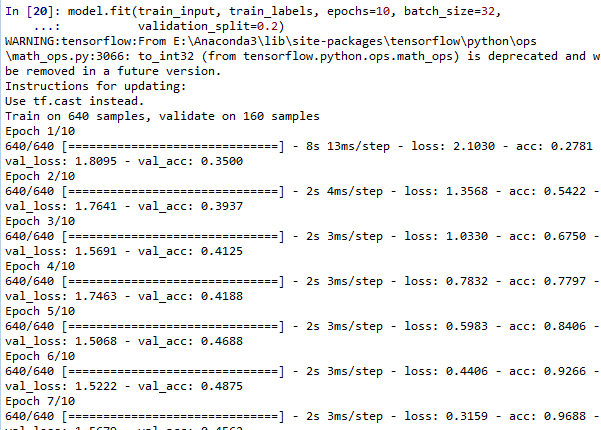
\includegraphics[scale=0.5]{figures/chapter6tasya19.png}
\caption{Fungsi Fit Tasya}
\label{Praktek}
\end{figure}
Dari hasil diatas dapat dijelaskan bahwa :
\begin{itemize}
\item Melakukan pelatihan dengan epoch atau iterasi dengan rambatan balik sebanyak 10, kemudian dalam sekali epochs dilakukan 32  sampel yang diproses sebelum model diperbarui.
\item Validation\_split sebesar 20\% untuk melakukan pengecekan pada cross score validation
\end{itemize}

\subsection{Fungsi Evaluate}
Berikut code lengkapnya : 
\lstinputlisting[caption=Code Fungsi Evaluate, label={lst:fungsievaluate}]{src/evaluate.tex}
Hasilnya seperti berikut :
\begin{figure}[ht]
\centering
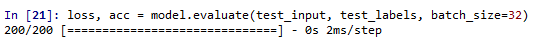
\includegraphics[scale=0.5]{figures/chapter6tasya20.png}
\caption{Fungsi Evaluate Tasya}
\label{Praktek}
\end{figure}
Dari hasil diatas dapat dijelaskan bahwa :
\begin{itemize}
\item Melakukan evaluasi atau  menemukan model terbaik yang mewakili data dan seberapa baik model yang dipilih akan bekerja di masa depan. Menggunakan test input dan test label.
\item Kemudian Hasilnya dapat dilihat seperti berikut :
\begin{figure}[ht]
\centering
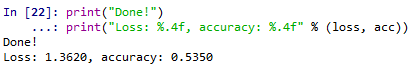
\includegraphics[scale=0.5]{figures/chapter6tasya21.png}
\caption{Fungsi Evaluate Tasya}
\label{Praktek}
\end{figure}
\item Dimana Loss yaitu hasil prediksi yang salah sebanyak 1,3620 dan keakurasian prediksinya yaitu 53\%
\end{itemize}

\subsection{Fungsi Predict}
Berikut code lengkapnya : 
\lstinputlisting[caption=Code Fungsi Predict, label={lst:fungsipredict}]{src/predict.tex}
Hasilnya seperti berikut : 
\begin{figure}[ht]
\centering
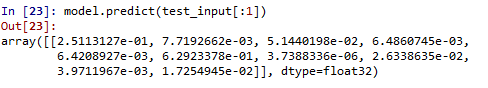
\includegraphics[scale=0.5]{figures/chapter6tasya22.png}
\caption{Fungsi Predict Tasya}
\label{Praktek}
\end{figure}
Dari hasil diatas dapat dijelaskan bahwa :
\begin{itemize}
\item Untuk melakukan prediksi diambil satu baris dari test\_input
\item Nilai yang tertinggi terdapat pada label kedua atau genre Classical
\item Untuk baris yang dipilih prediksi yang tepat yaitu lagu tersebut termasuk kedalam genre Classical
\end{itemize}

\section{Penanganan Error}
\subsection{Module Eror}
Berikut merupakan eror yang dijumpai ketika menjalankan skrip diatas
\begin{figure}[ht]
\centering
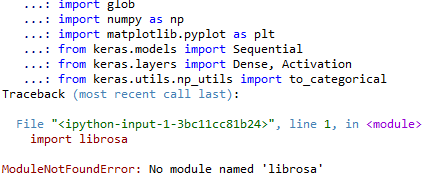
\includegraphics[scale=0.5]{figures/chapter6eror.png}
\caption{Module Error Tasya}
\label{Error}
\end{figure}
\begin{itemize}
\item Jenis error tersebut adalah ModuleNotFoundError : No Module named 'librosa' . Error ini terjadi dikarenakan target atau tujuannya tidak terinstall. Maka yang perlu dilakukan yaitu :
\begin{itemize}
\item Buka Anconda atau conda prompt
\item Ketikan 'conda install -c conda-forge librosa dan enter
\item Tunggu sampai proses instalasi berhasil
\item Jika Sudah, jalankan kembali skrip tadi maka hasilnya seperti berikut
\begin{figure}[ht]
\centering
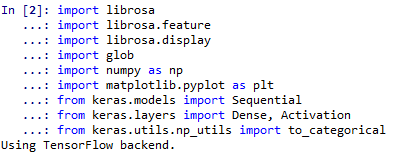
\includegraphics[scale=0.5]{figures/chapter6eror1.png}
\caption{Penyelesaian Module Error Tasya}
\label{Error}
\end{figure}
\item Tandanya eror sudah berhasil ditangani
\end{itemize}
\end{itemize}






